\documentclass{article}
\usepackage{tikz}
\usetikzlibrary{positioning}
\usepackage[margin=2cm]{geometry}

\begin{document}

% ---------- Schéma en étoile ----------
\section*{Schéma en étoile}

\noindent\makebox[\textwidth][c]{%
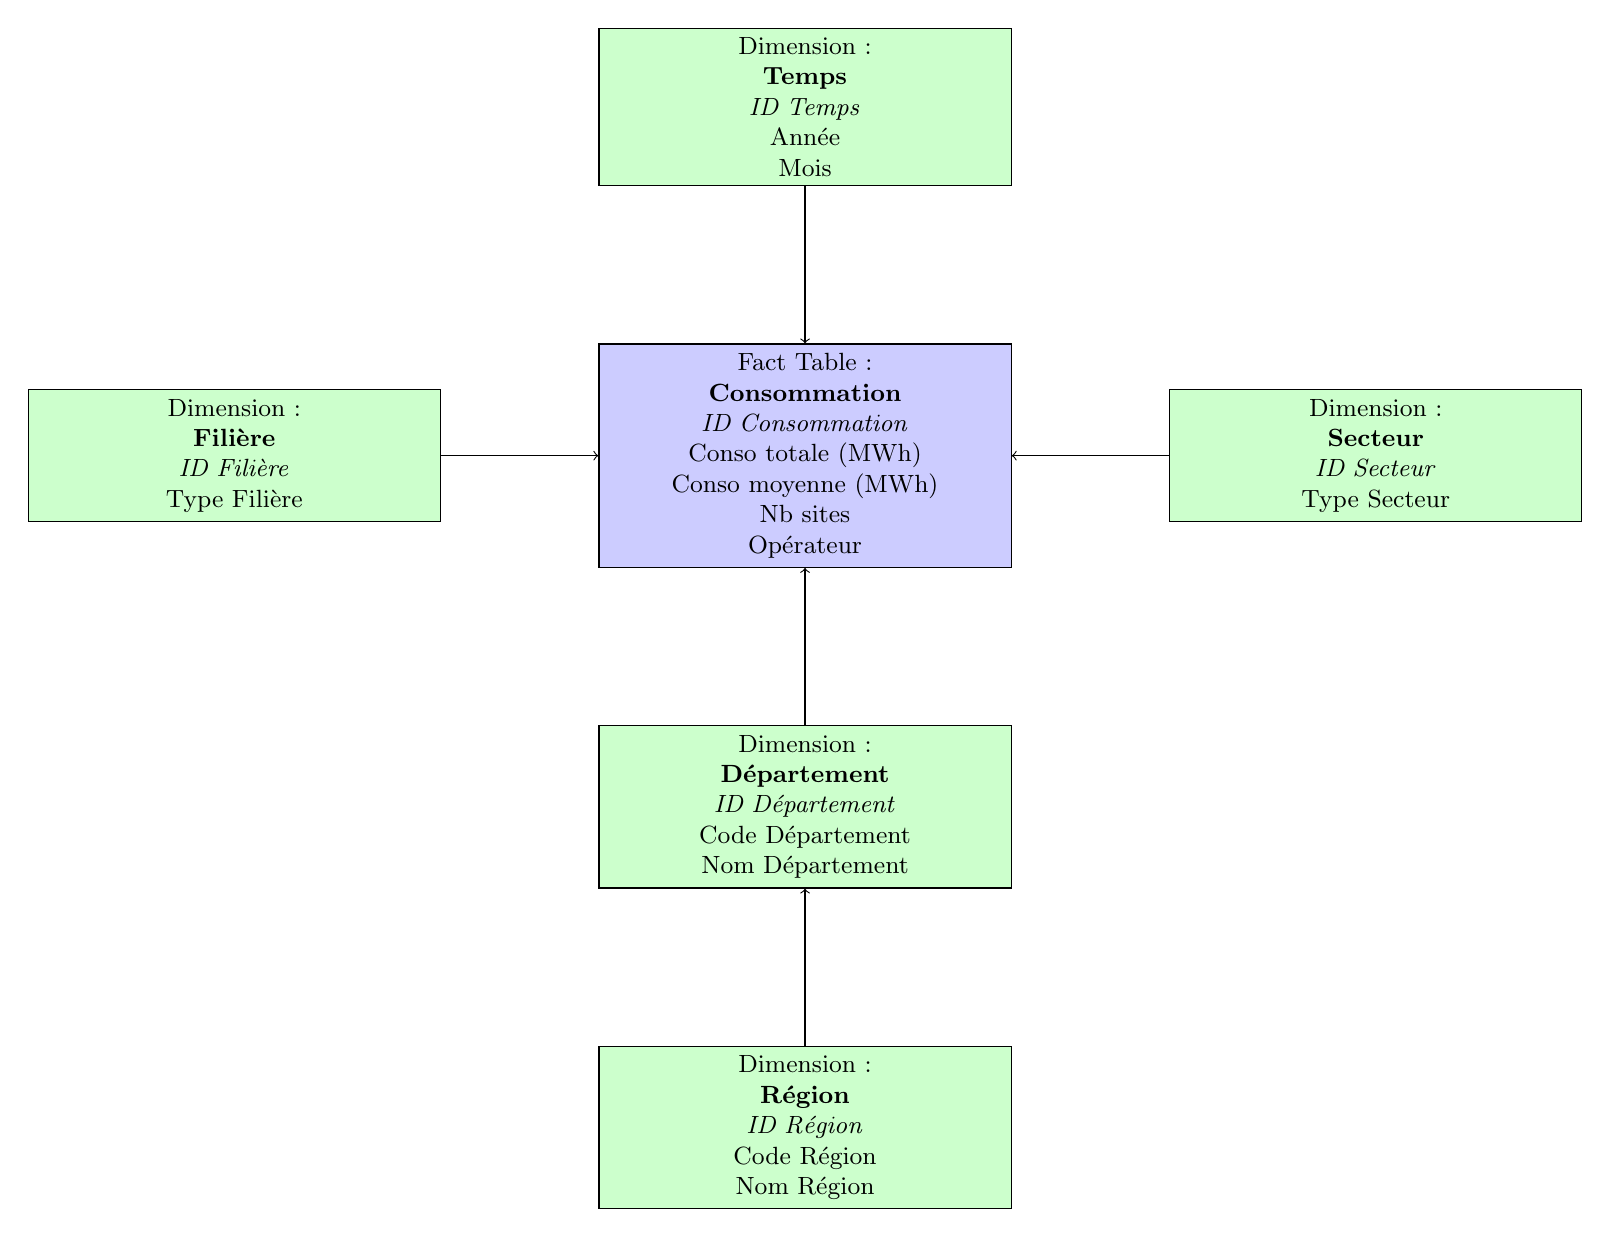
\begin{tikzpicture}[
    node distance=2cm,
    every node/.style={draw, text width=5cm, align=center, font=\small},
    fact/.style={fill=blue!20},
    dim/.style={fill=green!20}
]

% Table de faits
\node[fact] (consommation) {Fact Table :\\ \textbf{Consommation} \\
\textit{ID Consommation} \\
Conso totale (MWh) \\
Conso moyenne (MWh) \\
Nb sites \\
Opérateur};

% Dimensions
\node[dim, left=of consommation] (filiere) {Dimension :\\ \textbf{Filière} \\
\textit{ID Filière} \\
Type Filière};

\node[dim, above=of consommation] (temps) {Dimension :\\ \textbf{Temps} \\
\textit{ID Temps} \\
Année \\
Mois};

\node[dim, right=of consommation] (secteur) {Dimension :\\ \textbf{Secteur} \\
\textit{ID Secteur} \\
Type Secteur};

\node[dim, below=of consommation] (departement) {Dimension :\\ \textbf{Département} \\
\textit{ID Département} \\
Code Département \\
Nom Département};

\node[dim, below=of departement] (region) {Dimension :\\ \textbf{Région} \\
\textit{ID Région} \\
Code Région \\
Nom Région};

% Liens
\draw[->] (filiere) -- (consommation);
\draw[->] (temps) -- (consommation);
\draw[->] (secteur) -- (consommation);
\draw[->] (departement) -- (consommation);
\draw[->] (region) -- (departement);

\end{tikzpicture}%
}

\vspace{2cm}

\section*{Schéma relationnel}

\begin{itemize}
    \item \textbf{Consommation}(\underline{ID\_Consommation}, ID\_Filiere, ID\_Temps, ID\_Secteur, ID\_Département, Conso\_Totale, Conso\_Moyenne, Nb\_Sites, Opérateur)
    
    \item \textbf{Filière}(\underline{ID\_Filiere}, Type\_Filiere)
    
    \item \textbf{Temps}(\underline{ID\_Temps}, annee)
    
    \item \textbf{Secteur}(\underline{ID\_Secteur}, Type\_Secteur)
    
    \item \textbf{Département}(\underline{ID\_departement},  code\_departement, Nom\_departement, ID\_region)
    
    \item \textbf{region}(\underline{ID\_region}, code\_region, nom\_region)
\end{itemize}

\end{document}
